\chapter{Results}
\label{ch:results}

The results reported are calculated over the dedicated testing set of $60$ scans. It was measured metrics, $Id rate$, $mean localization distance$ and $standard deviation (std) distance$. $Id rate$ is the percentage of the centroid estimations predicted which are closest to the correct ground truth vertebra centroid (and are less than $20mm$ from that centroid). $Mean$ and $Std$ relate to the localization error distance between the predicted centroid positions and the ground-truth centroid positions for the same vertebrae (if it occurs at the scan). 

Table \ref{results_table} represents a performance of the method.
It performs slightly worse on the Id rate. A possible reason for this is that our method relies on the ordering of vertebrae and sufficient contextual information to localize in a dense regression identification stage, but it does not explicitly classify vertebrae, for example, using categorical cross entropy. 

\begin{figure}[!h]
\begin{center}
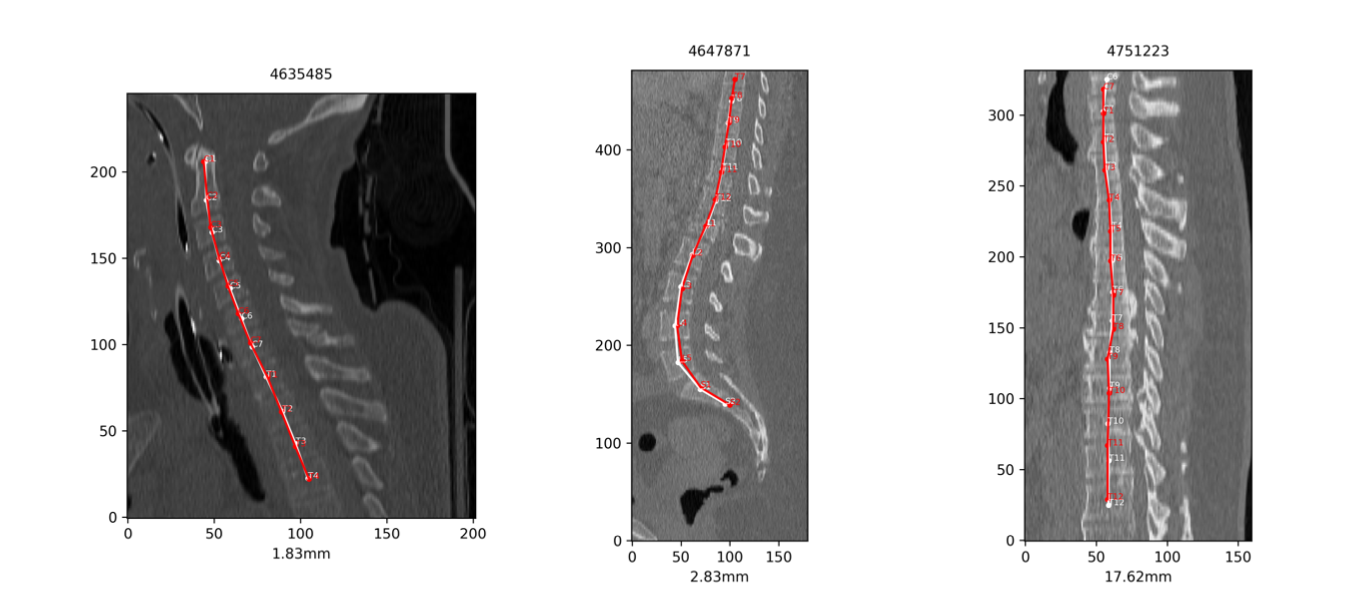
\includegraphics[width=.5\linewidth]{images/3_predictions.png}
\caption {Example of 3 predictions, the red points are method’s centroid predictions, the white points are the ground-truth centroid locations, below each scan the mean localization error for that scan is shown as well.} 
\label{fig:3_predictions}
\end{center}
\end{figure}

The advantage of the method is that it is lightweight and fast both in training time, models took $> 11 hours$ (detection model) and $> 7 hours$ (identification model) to train, but also at test time, with predictions for a scan being computed on average in $40 seconds$. The method does not rely on an iterative stage and usage of RNN, thus making the method likely more efficient at test time.

\begin{center}\label{results_table}
\begin{tabular}{ c c c }
 ID rate & Mean & Std \\ 
 85.8\% & 5.60 & 7.10 \\  
 90.6\% & 3.93 & 5.27 \\
 79.8\% & 6.61 & 7.40 \\
 92.0\% & 5.39 & 8.70 \\
\end{tabular}
\end{center}


